\documentclass[a0,landscape]{a0poster}
\usepackage{helvet} % Use Helvetica as the sans-serif font
\usepackage{graphicx}
\usepackage{geometry}
\usepackage{qrcode}
\usepackage{amssymb}
\usepackage{alltt}
\usepackage{tikz}
\usetikzlibrary{shapes.geometric, arrows.meta}

% --- Set sans-serif as the default font family ---
\renewcommand{\familydefault}{\sfdefault}

% --- Page Geometry (48x36 inches with a 1-inch margin) ---
\geometry{papersize={48in,36in}, margin=1in, top=1.5in}

\begin{document}

% === GRADIENT BACKGROUND ===
\begin{tikzpicture}[remember picture, overlay]
    \shade[top color=blue!10, bottom color=blue!25, middle color=blue!15]
    (current page.south west) rectangle (current page.north east);
\end{tikzpicture}

% === NEW HEADER BLOCK (Title on left, QR code on right) ===
\begin{minipage}[c]{0.78\linewidth}
    \Huge \textbf{A Software Tool for Planning Better Clinical Trials} \\ %\vspace{3cm}
    \huge \textbf{Arnab Aich, Yuan Zhang} \\
    \Large \textit{Department of Preventive Medicine, University of Tennessee Health Science Center}
\end{minipage}
\hfill
\begin{minipage}[c]{0.2\linewidth}
    \begin{center}
        \qrcode[height=4.5cm]{https://github.com/UTHSC-Zhang/RMSTSS-Package}
    \end{center}
\end{minipage}

\vspace{0.5cm}
\rule{\linewidth}{1.5pt}
\vspace{1cm}


% === TWO-COLUMN LAYOUT START ===

\begin{minipage}[t]{0.44\linewidth}

    \subsection*{\huge Key Questions in Clinical Trials}
    \begin{center}
        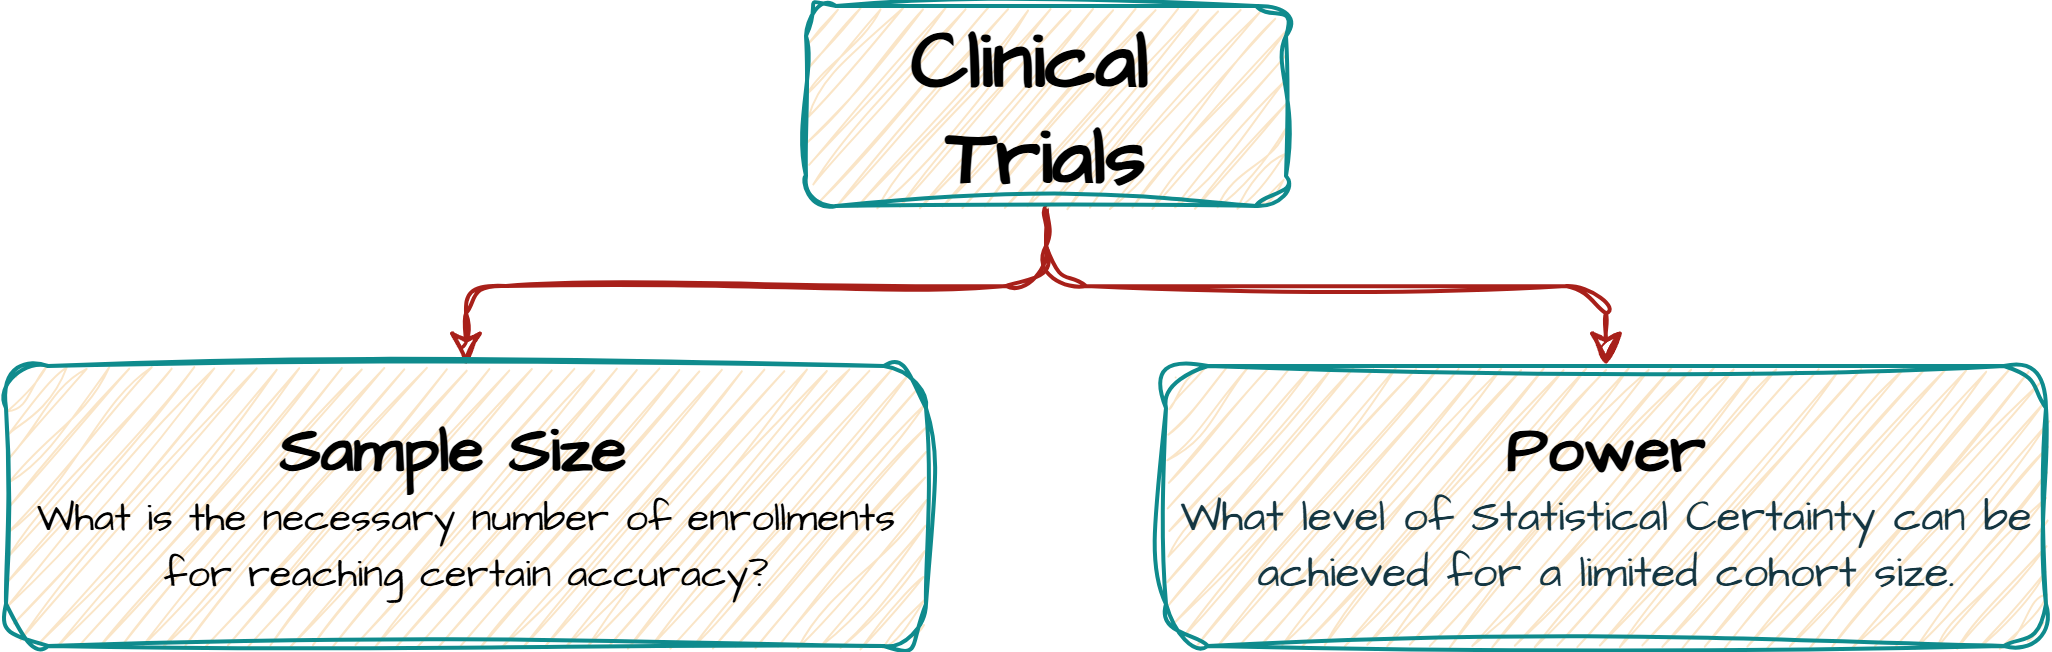
\includegraphics[width=\linewidth]{images/diag-CT.png}
    \end{center}

    \subsection*{\Large Problems in Traditional Methods}
    \large For decades, Survival trials (\textit{Time to event}) have relied on the \textbf{HR} (Hazard Ratio).
    \begin{itemize}
        \item[\large\checkmark] This metric depends on strong assumptions that are often violated in the real world.
        \item[\large\checkmark] Can't identify treatment benefits.
    \end{itemize}
    \subsection*{\Large Our Solution: RMST}
    \large We use \textbf{RMST} (Restricted Mean Survival Time), which directly measures the average \textbf{event-free} time patients experience.
    \begin{itemize}
        \item[\large\checkmark] It is easy for everyone to understand.
        \item[\large\checkmark] It provides a clear measure of treatment benefit.
    \end{itemize}
    \begin{center}
        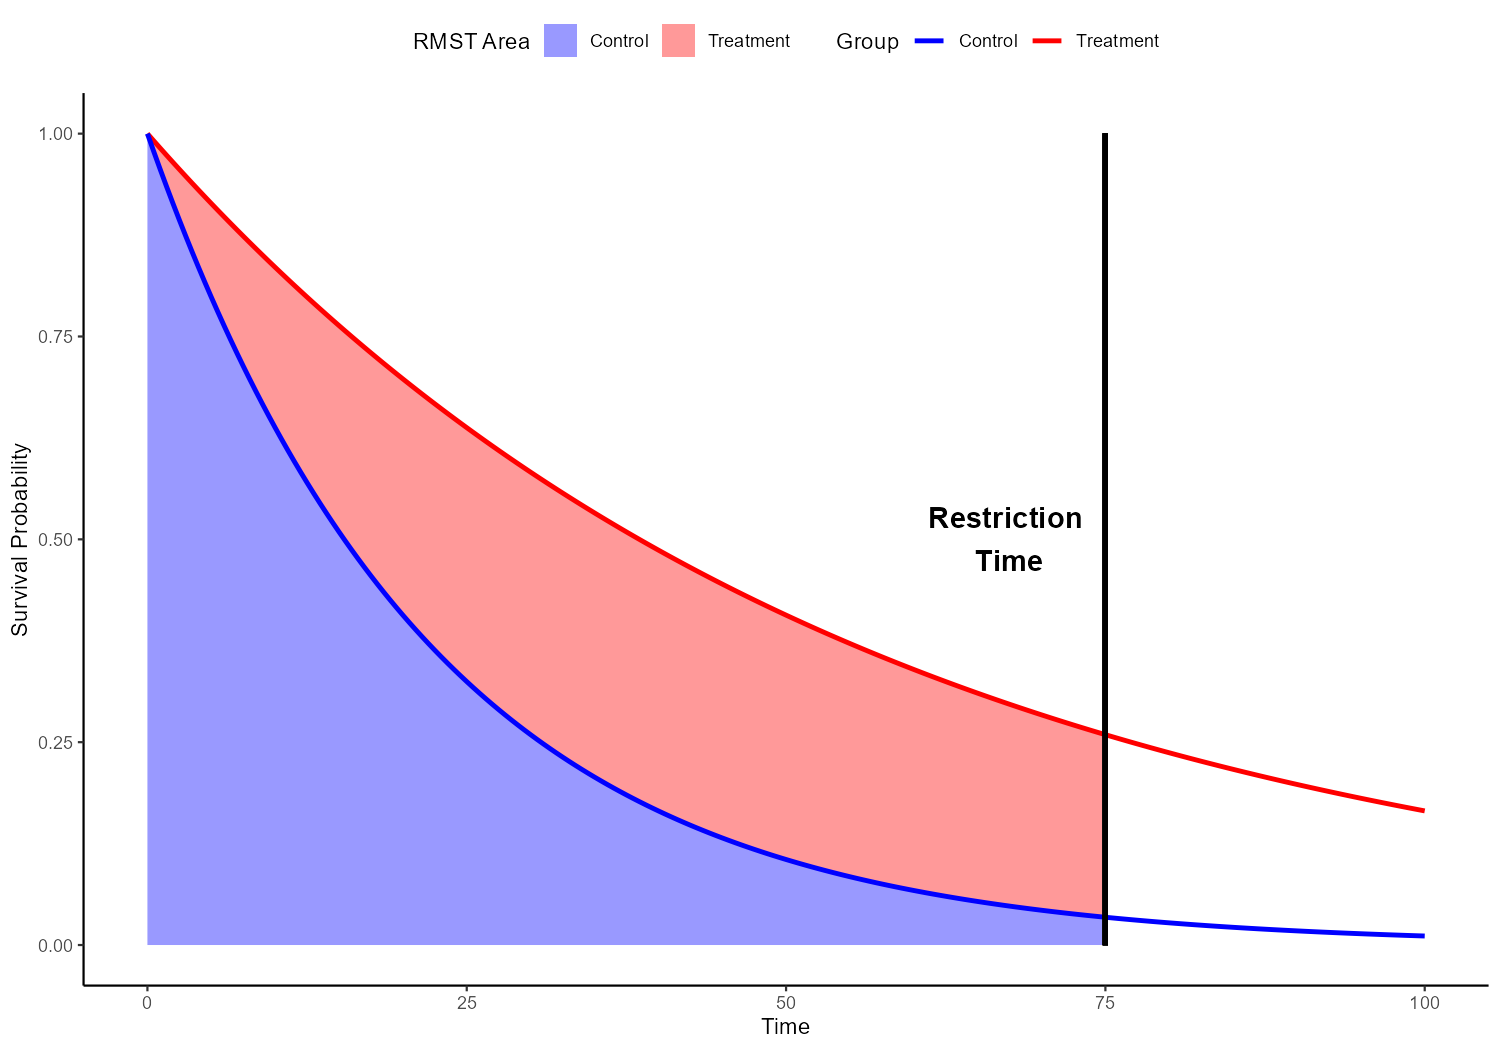
\includegraphics[width=\linewidth,height = 0.5\linewidth]{images/rmst_causal_plot.png}
    \end{center}
\end{minipage}
\hfill
\begin{minipage}[t]{0.54\linewidth}
    % --- COLUMN 2: THE RMSTSS TOOL ---
    \subsection*{\huge What We Are Offering}
%    \Large ‘RMSTSS‘ is a free tool that helps researchers properly plan modern medical studies.
    \begin{center}
        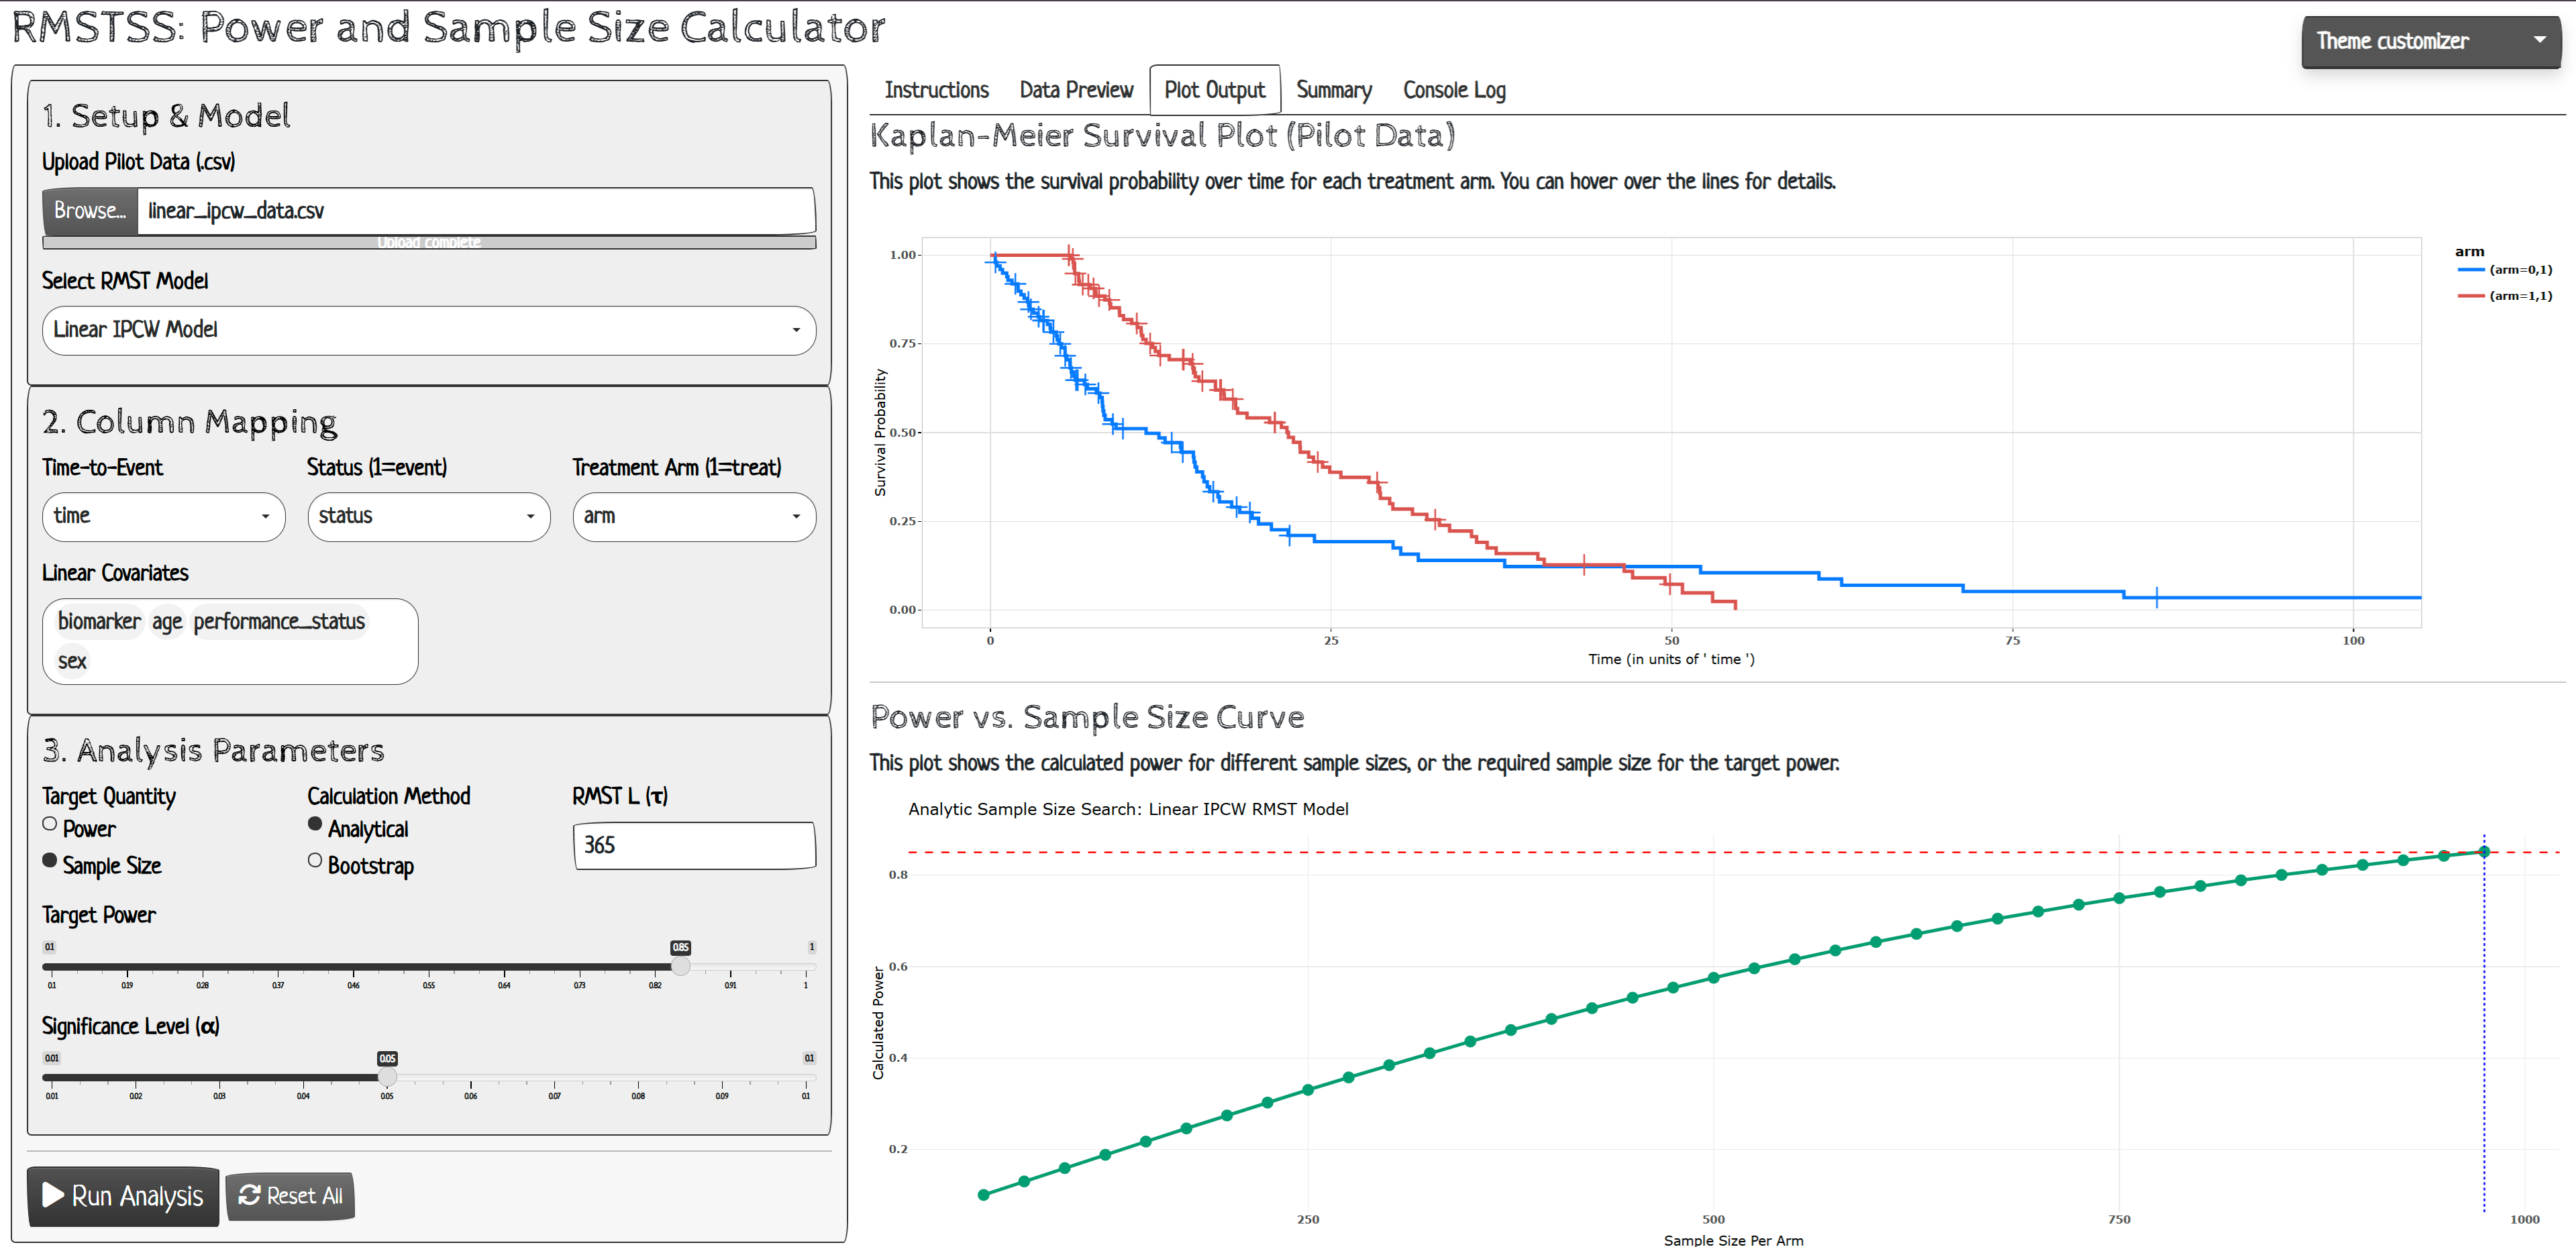
\includegraphics[width=\linewidth]{images/app-ss.png}
    \end{center}
    \subsection*{\Large App Features}
    \begin{itemize}
        \item \large \textbf{Variable Selection:} Choose variables to add in model.
        \item \large \textbf{Flexible Methods:} Use a \textbf{Quick Check} (Analytical) or a \textbf{Deep Dive}(Bootstrap).
        \item \large \textbf{Downloadable Reports:} Generate an HTML report for documenting purposes.
        \item \large \textbf{Customization:} Change themes, fonts, size, and many more on the go.
    \end{itemize}
    
    \begin{center}
        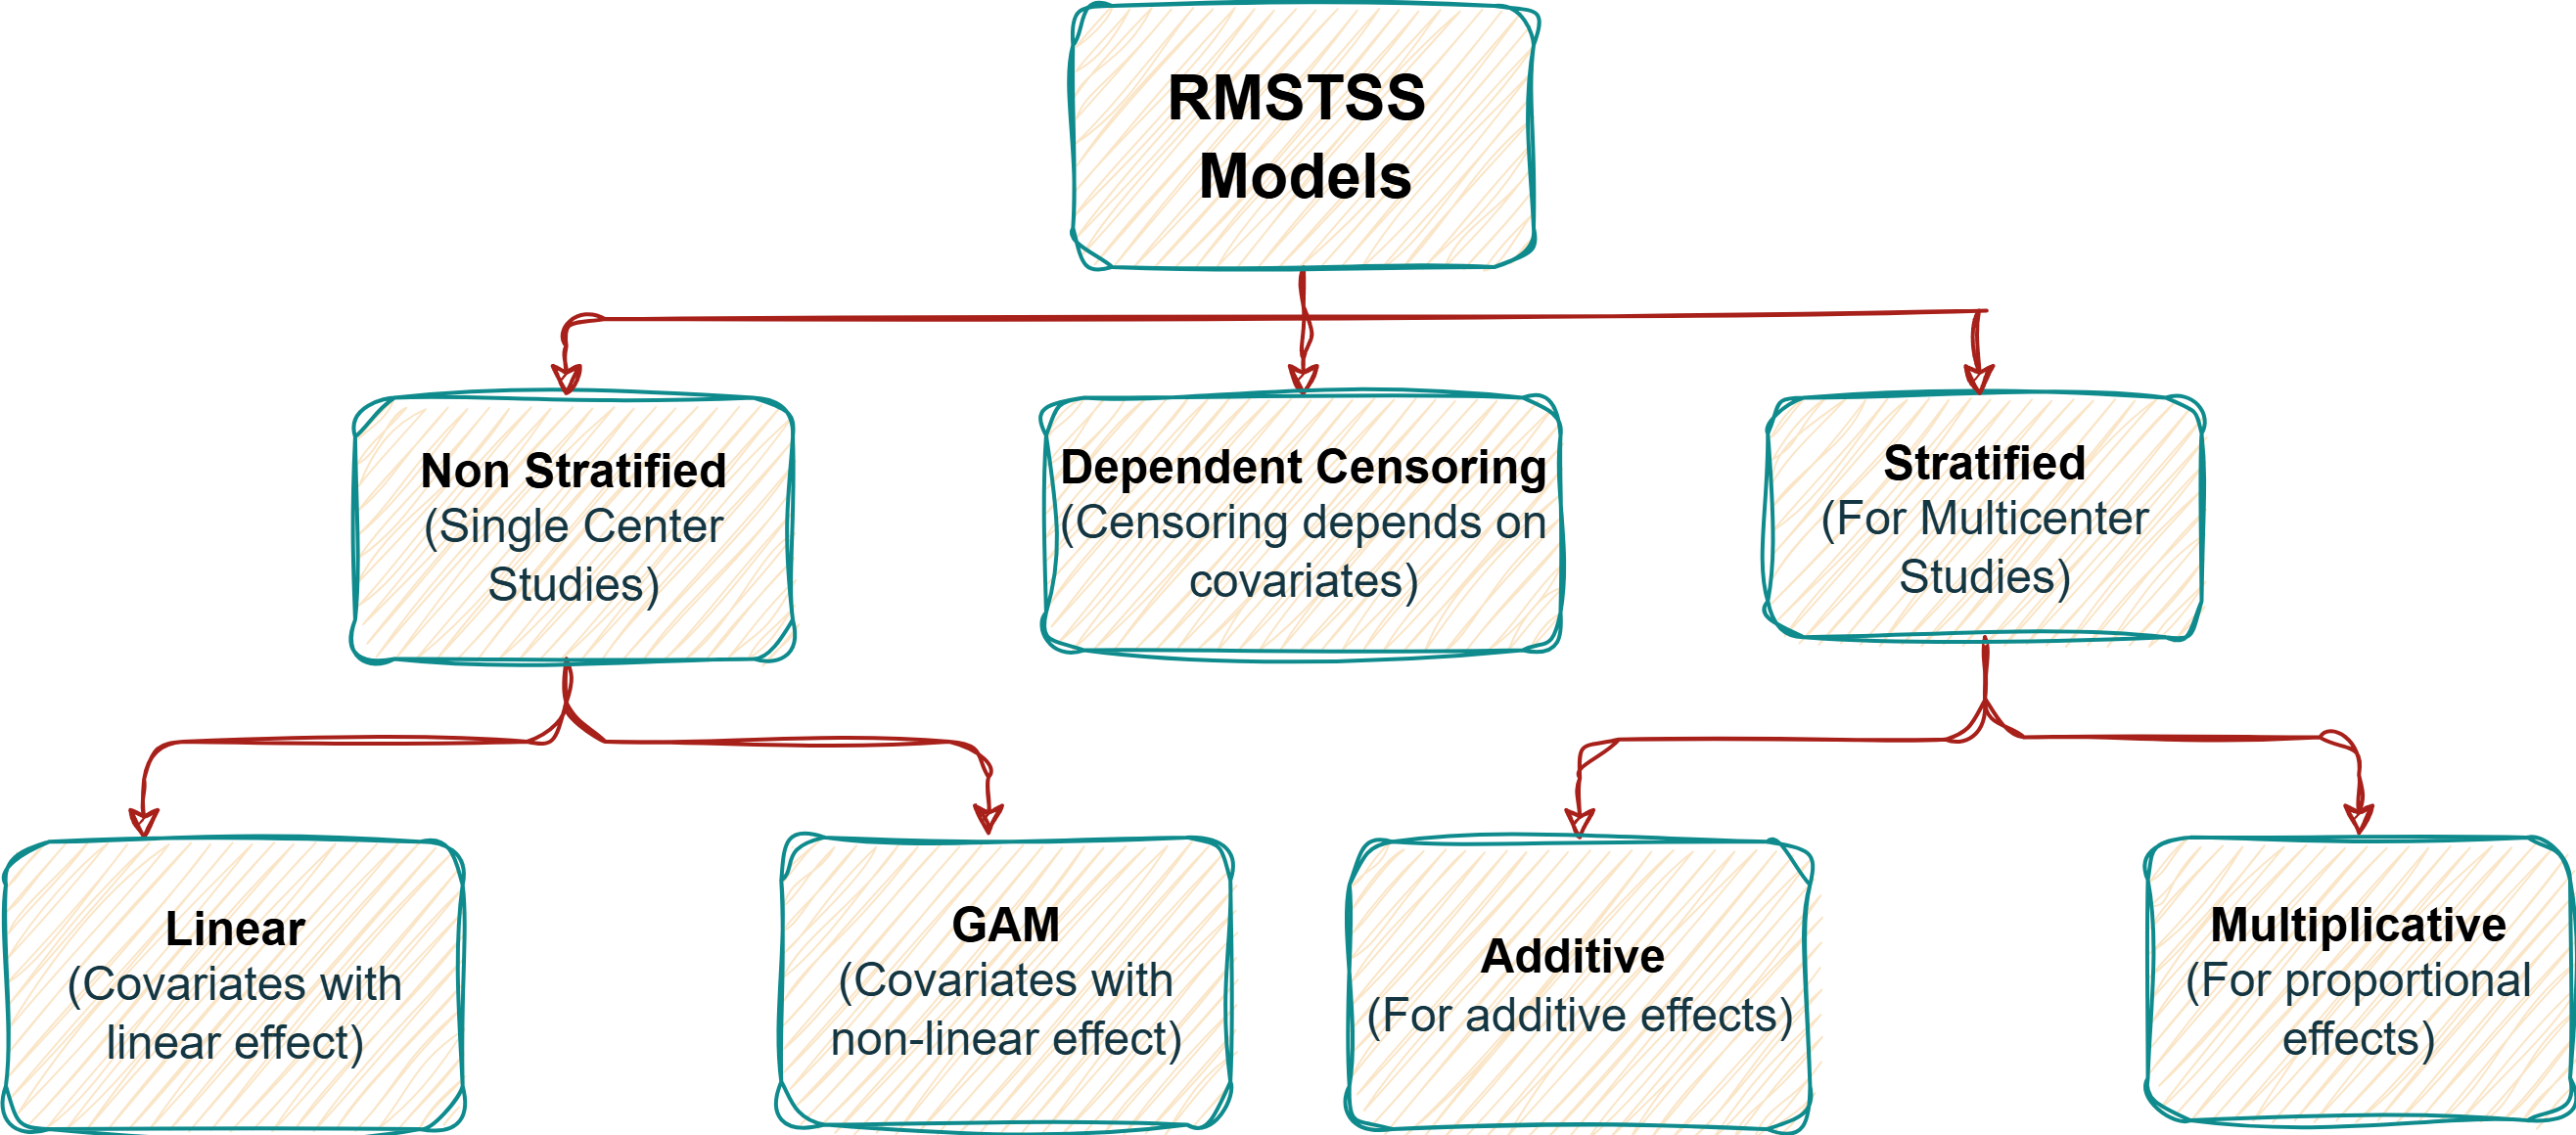
\includegraphics[width=\linewidth,height = 0.4\linewidth]{images/app-models.png}
    \end{center}
    
\end{minipage}

\hfill

\rule{\linewidth}{1pt} % Horizontal line to separate footer

\begin{minipage}[t]{0.5\linewidth}
    \subsection*{\Large For Statisticians and Programmers}
    \large We also developed an \textbf{R-Package} for function-level interaction. After installing the package from GitHub, the app can be run locally using the \verb|RMSTSS::run_app()| function call. For the package website scan the QR code.
\end{minipage}
\hfill
\begin{minipage} {0.2\linewidth}
\vspace{0.5cm}
    \begin{center}
        \qrcode[height=4.6cm]{https://github.com/UTHSC-Zhang/RMSTSS-Package}
    \end{center}
\end{minipage}
\hfill
\begin{minipage}[t]{0.25\linewidth}
    \subsection*{\Large Acknowledgments}
    \begin{enumerate}
        \item NSF grant no. 2220726.
        \item UTHSC BERD (Biostatistics, Epidemiology and Research Design).
    \end{enumerate}
\end{minipage}

% === LAYOUT END ===

\end{document}